\documentclass[unknownkeysallowed]{beamer}

\mode<presentation> {

\usetheme{Madrid}

}

\usepackage{graphicx} % Allows including images
\usepackage{booktabs} % Allows the use of \toprule, \midrule and \bottomrule in tables

\usepackage[slovene]{babel}
\usepackage[utf8]{inputenc}

\usepackage{algorithmicx, algpseudocode}

\usepackage{varwidth}

\algrenewcommand\alglinenumber[1]{\scriptsize #1:}

\renewcommand{\algorithmicrequire}{{\bf Vhod:}}

\def\R{\mathbb R}
\def\N{\mathbb N}

%----------------------------------------------------------------------------------------
%	TITLE PAGE
%----------------------------------------------------------------------------------------

\title[Text Analysis]{Text classification using persistent homology} % The short title appears at the bottom of every slide, the full title is only on the title page

\author{Domen Keglevič, Matija Čufar} % Your name
\institute[] % Your institution as it will appear on the bottom of every slide, may be shorthand to save space
{
Faculty of Computer and Information Science \\ % Your institution for the title page
\medskip
}
\date{\today} % Date, can be changed to a custom date

%----------------------------------------------------------------------------------------
%	PRESENTATION
%----------------------------------------------------------------------------------------

\begin{document}

\begin{frame}
\titlepage % Print the title page as the first slide
\end{frame}

\begin{frame}
\frametitle{Problem description} 
\begin{block}{Problem}
\begin{columns}[c]
\column{.6\textwidth}
	Given sets of texts from different domains, build a classifier which can distinguish between the domains.

\column{.35\textwidth}
	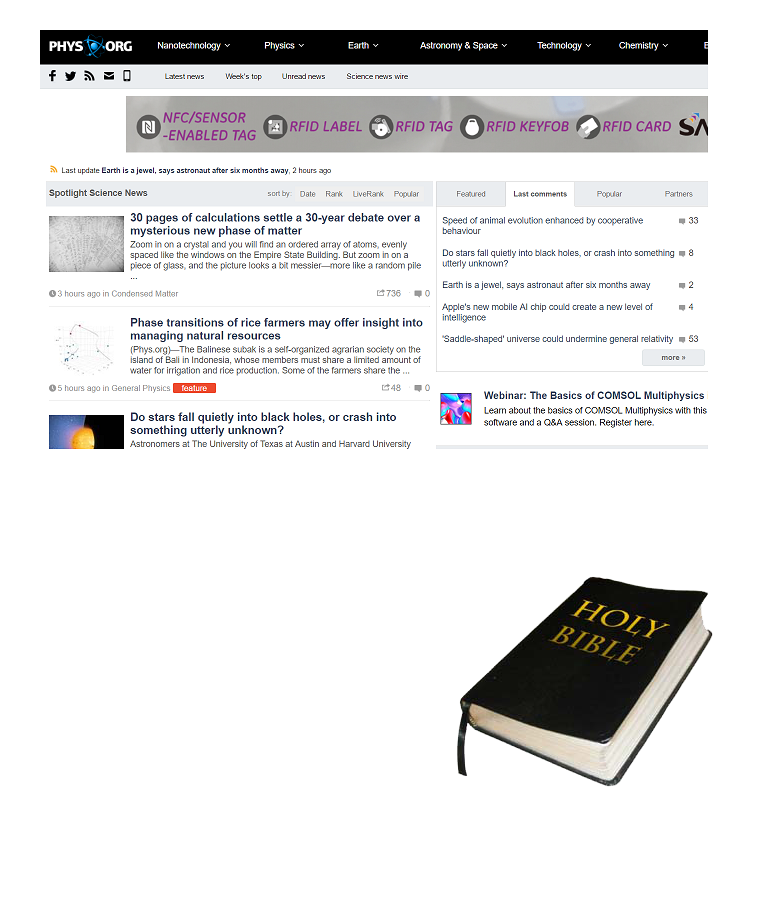
\includegraphics[width=0.9\linewidth]{different_domains}
\end{columns}
\end{block}

\end{frame}


\begin{frame}
\frametitle{Solution idea}
\begin{columns}[c]
\column{.5\textwidth}
	\begin{itemize}
		\item Use persistent homology.
		\medskip
	\end{itemize}
\column{.5\textwidth}
	
\end{columns}
\end{frame}

%------------------------------------------------

\begin{frame}{The End}
\Huge{\centerline{The End}}
\end{frame}

%----------------------------------------------------------------------------------------

\end{document}